\documentclass[jou,a4paper,notxfonts]{apa}
\usepackage{graphicx} 
\usepackage{palatino}
\usepackage{fancyhdr}
\usepackage{url}
\pagestyle{fancy}



% header on first page
\fancypagestyle{plain}{%
\fancyhf{} % clear all header and footer fields
\fancyhead[L]{\small
Journal of Eye Movement Research\\
1(1):1, 1-2}
\fancyfoot[C]{\thepage}
\renewcommand{\headrulewidth}{0pt}
\renewcommand{\footrulewidth}{0pt}}



\title{Distributed Eye Tracking Network for Conveying Population Gaze in a Robotic Telepresence Scenario} %Fill this in


%please refer to http://www.ilsp.gr/homepages/protopapas/apacls.html#titlhead for different numbers of authors and affiliations
\threeauthors{First Author}{Second Author}{Third Author}
\threeaffiliations{First affiliation}{Second Affiliation}{Third Affiliation}


\journal{}
\volume{}

\abstract{Robot based telepresence technology allows one or several remote users to visit a distant geographical
location using a mobile robot. The robot can carry a 360$^\circ$ panoramic camera that provides to the remote users an
immersive viewing perspective of the robot environment through a video live stream. One limitation of this technology is
that for humans around the robot or elsewhere, is difficult to gather a sense of where in the robot's environment the
remote users are paying attention to. These contrasts sharply with physical presence where body language and other
subtle cues provide a hint of where the person is paying attention to. Here, we propose the usage of a distributed
network of eye trackers to monitor the gaze behavior and field of view of the remote users of the robotic telepresence
system. This information can be mapped to a 3D point in space in order to track where in the environment surrounding the
robot the remote users are paying attention to.  This information can be send back to the robot that then superimposes
the aggregated gaze behavior of the remote users in a condensed 2D representation of the panoramic image it is currently
capturing from the environment. We use as an illustrative application, a robot being employed to visit a museum remotely
by several high school students distributed across Australia. A human museum guide, directs the robot around the museum
while explaining and interacting with the remote students through the visual display on the robot. The visualization of
the gaze behavior of the remote students in real time provides a useful feedback signal to the museum tour guide about
where the remote students are paying attention in the guide environment so he or she can adapt his or her behavior
accordingly.
\linebreak
\linebreak
{\bf Keywords: eye tracking, gaze tracking, telepresence, eye tracking network, gaze aware interfaces, pervasive
computing, HCI, gaze responsive interfaces, human computer interaction}}

\acknowledgements{}
\shorttitle{}
\rightheader{}

% repeat the authors here (use et al if more than three authors):
\leftheader{ }

\begin{document}

\maketitle

\lhead{\small
Journal of Eye Movement Research\\
1(1):1, 1-2
}
\rhead{
Author, A., Author, B., & Author, C. (2007)\\
Short Title
}
\thispagestyle{plain}

\section{Introduction} 
Telepresence technology allows a person to feel and/or to have an effect as if they were present at a place other than
their real location. Telepresence technology requires that the remote user is provided with sensory stimuli conveying
information about the distant location in order to re-create the feeling of being in that other location. This is
usually done by visual and audio sensors that capture and transmit the information about an environment to the remote
users. The option of interacting with the remote location through output effectors can be give to the remote users. This
can be achieved by sensing, transmitting and duplicating in the remote location the user's position, movements, actions,
or voice. Hence, in realistic telepresence sytems, information flows in both directions between the distant locations.
Telepresence systems enable collaboration independent of geographic location and provide considerable savings in terms
of time, travel cost and environmental impact for numerous usage scenarios. 


A robotic telepresence can allow a subject to move virtually through a distant building by remotely controlling a
wheeled robot equipped with a camera, microphone, loudspeaker. An screen in the mobile robot can optionally display
live video of the subject�s face allowing the remote users to interact with subjects around the robot. Telepresence
systems range of possible uses have increase considerably in the last years thanks to advances in robotics and
telecommunication technologies.


In this work, we augment an existing telepresence system that allows remote visitors to visit a museum using a semi
autonomous mobile robot and an immersive web interface. The system is designed to allow remote visitors to feel as they
are on an actual tour in the museum  by employing a web browser viewer of the panoramic video streamed by the robot.
The innovative part of the system is the usage of a network of eye trackers that monitor the gaze behavior of the
museum visitors and transmits the gaze data to the mobile robot. The robot can then displays on its on-board 
screen the gaze behavior of the remote users in order to provide to the educator at the museum with information about
what is attracting the gaze (and hence the attention) of the remote students.


The point of regard (PoR) of a computer user on the screen can be estimated using video oculography gaze tracking. The
usage of eye gaze as a pointing or control mechanism is well documented in the literature
\cite{duchowski, Rozado2012, Bonino2011, danhansenrevieweyetrackingmethods}. Gaze tracking has found a niche application
to study how computer users interact with content on a computer screen \cite{Rozado2012a, giaet, myiwann2011}. The gaze
data accumulated during a gaze tracking session can be visualized off-line as a heat map data structure. A heat map
captures the accumulated degree of attention that a given user places at different points on the screen during the gaze
tracking trial. Hence, it is well-established that the direction of gaze reflects the user's focus of attention on the
screen \cite{Zhai2003}, and hence, it provides a hint about intention. In this work, we leverage on these well known
facts about eye tracking practice and extend it to a network of eye trackers scenario that work together to convey the
gaze behavior of several remote museum visitors in a remote telepresence systems.

% Literature review
The concept of telepresence systems is not new. The work from \cite{minsky1980telepresence} coined the term
\emph{telepresence} to describe systems that would transform work, manufacturing, energy production and medicine. Minsky
proposed the idea of being able to work in another country or planet through remote telepresence.

One of the first and most popular applications of telepresence is videoconferencing \cite{duncanson1973video}. The
review  from \cite{Egido:1988:VCT:62266.62268} highlighted some of the limitations of the technology at the time it was
first proposed, most of which have already been overcome \cite{lawson2010images}.

Another branch of telepresence that has gathered a lot of attention in the research literature is telesurgery, also
known as \emph{surgery at a distance} \cite{green1995telepresence}. The technique allows surgeons to operate
robotically on a patient that is located in different geographical coordinates. Among the many benefits of
the telesurgery concept, the technology has the potential to revolutionize healthcare delivery by bringing surgical
attention to previously inaccessible settings \cite{holt2004telesurgery}.


More recently, telepresence robots that are controlled remotely and allow a human to explore remote graphical location
have been proposed \cite{schultz1991telepresence} and have received a considerable amount of research attention
\cite{tsui2011exploring}.


An important feature of robotic telepresence systems is their ability to realistically capture their surrounding
environment in order to convey a realistic representation of their location to the remote users. Panoramic images are a
key component of many modern Robotic telepresence systems to provide the functionality of capturing and transmitting a
high quality visual representation of the robot's surrounding environment. The work from \cite{Gledhill2003435} provides
a good overview of panoramic imaging technologies summarizing and comparing some of the methods to carry out capturing,
image processing, image stitching, 3-D reconstruction, rendering and visualization.


Gaze tracking has been used extensively to monitor the gaze behavior of subjects in a variety of circumstances and
environments \cite{duchowski, jacob2003eye, myiwann2011}. However, to our knowledge, there is no literature available on
the utility of using gaze tracking to transmit the gaze behavior of remote users to the robotic environment in a
telepresence system. The amount of literature on using networks of eye trackers is also very limited due to their high
cost of the devices until very recently.


In Summary, in this work, we augment a robotic telepresence system that allows live interaction between remote students
and an educator in a museum by adding gaze tracking of the remote users.  Multiple remote museum visitors connect via a
single robot to the museum telepresence tour, but each remote visitor controls their own view within the gallery. Remote
students can access additional digital content about objects on display augmenting thereby the tour experience. A
network of eye trackers in the remote students' computers monitor and transmit their gaze behavior. This gaze behavior
data is displayed in the robot screen to provide feedback signal to museum tour guide about where the remote visitors
are paying attention to. This information closes the interaction loop between the educator in the museum and the remote students
and offsets some of the nonverbal communication limitations of telepresence systems by signaling to the museum tour
guide where the remote museum visitors are paying attention to at any given instant in time.


%XXXXXXXXXXXXXXXXXXXXXXXXXXXXXXXXXXXXXXXXXXXXXX
\section{Method}
The entire gaze monitoring and robotic telepresence system comprises several subparts that we described below.

\subsubsection{Eye-tracking system}
Eyes are used by humans to obtain information about the surroundings and to communicate information. When something
attracts our attention, we position our gaze on it, thus performing a \emph{fixation}. A fixation usually has a
duration of at least 150 milliseconds (ms). The fast eye movements that occur between fixations are known as
\emph{saccades}, and they are used to reposition the eye so that the object of interest is projected onto the fovea.
The direction of gaze thus reflects the focus of \emph{attention} and also provides an indirect hint for
\emph{intention}\cite{velichkovsky}.


A video-based gaze tracking system seeks to find where a person is looking, i.e. the Point of Regard (PoR), using images
obtained from the eye by one or more cameras. Most systems employ infrared illumination that is invisible to the human
eye and hence it is not distracting for the user. Infrared light improves image contrast and produces a reflection on
the cornea, known as corneal reflection or glint. Eye features such as the corneal reflections and the center of the
pupil/iris can be used to estimate the PoR. Figure \ref{screenGazeTracker} shows a screenshot of an eye being tracked by
the open-source ITU Gaze Tracker \cite{lowcostitugazetracker,Rozado2012}. In this case, the center of the pupil and two
corneal reflections are the features being tracked.


\begin{figure}[tp]
 %\fitbitmap[scale=0.5]{figures/screenGazeTracker.jpg}
 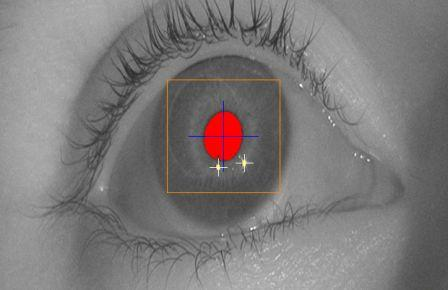
\includegraphics[width=0.45\textwidth, height=40mm]{figures/screenGazeTracker.jpg}
 \caption{\textbf{The Open Source ITU Gaze Tracker Tracking One Eye.} The
  features being tracked in the image are the pupil center and two corneal reflections. These features are used by the
  gaze estimation algorithms to determine the PoR of the user on the screen.}
 \label{screenGazeTracker}
\end{figure}

In most eye tracking studies, the PoR of the user is employed to generate a heat map of the scene observed or as a
pointing device that substitutes the mouse in gaze interaction paradigms. For this work, eye tracking was used behind
the scenes just to capture the gaze behavior of the remote museum visitors and transmit it to the robot in order for it
to display the aggregated gaze behavior of several users to the museum educator.

A set of 3 Tobii Rex eye trackers and 1 Tobii X1 light eye tracker are used for the experimental part. Both systems
track gaze at 30 frames per second (fps) with an average gaze estimation accuracy of 0.5 degrees at 60cm from the screen, 
\cite{TobiiTechnologyAB}. A simple exponential smoothing filter, \cite{Kumar2007}, of the raw gaze tracking data is
carried out to prevent jitter in the visualization of gaze.


\subsection{Robot}
% Fred, maybe you could provide more specific and technical details about this part?
We use a commercial robot that carries a head-height omnidirectional camera and a display screen, see
Figure \ref{MuseumRobot} to observe an early prototype of the system. The robot also carries a forward-looking camera
for video conferencing purposes between the museum tour guide and the remote students, two onboard computers and Wi-Fi
antennas.

\begin{figure}[tp]
 \begin{center}
 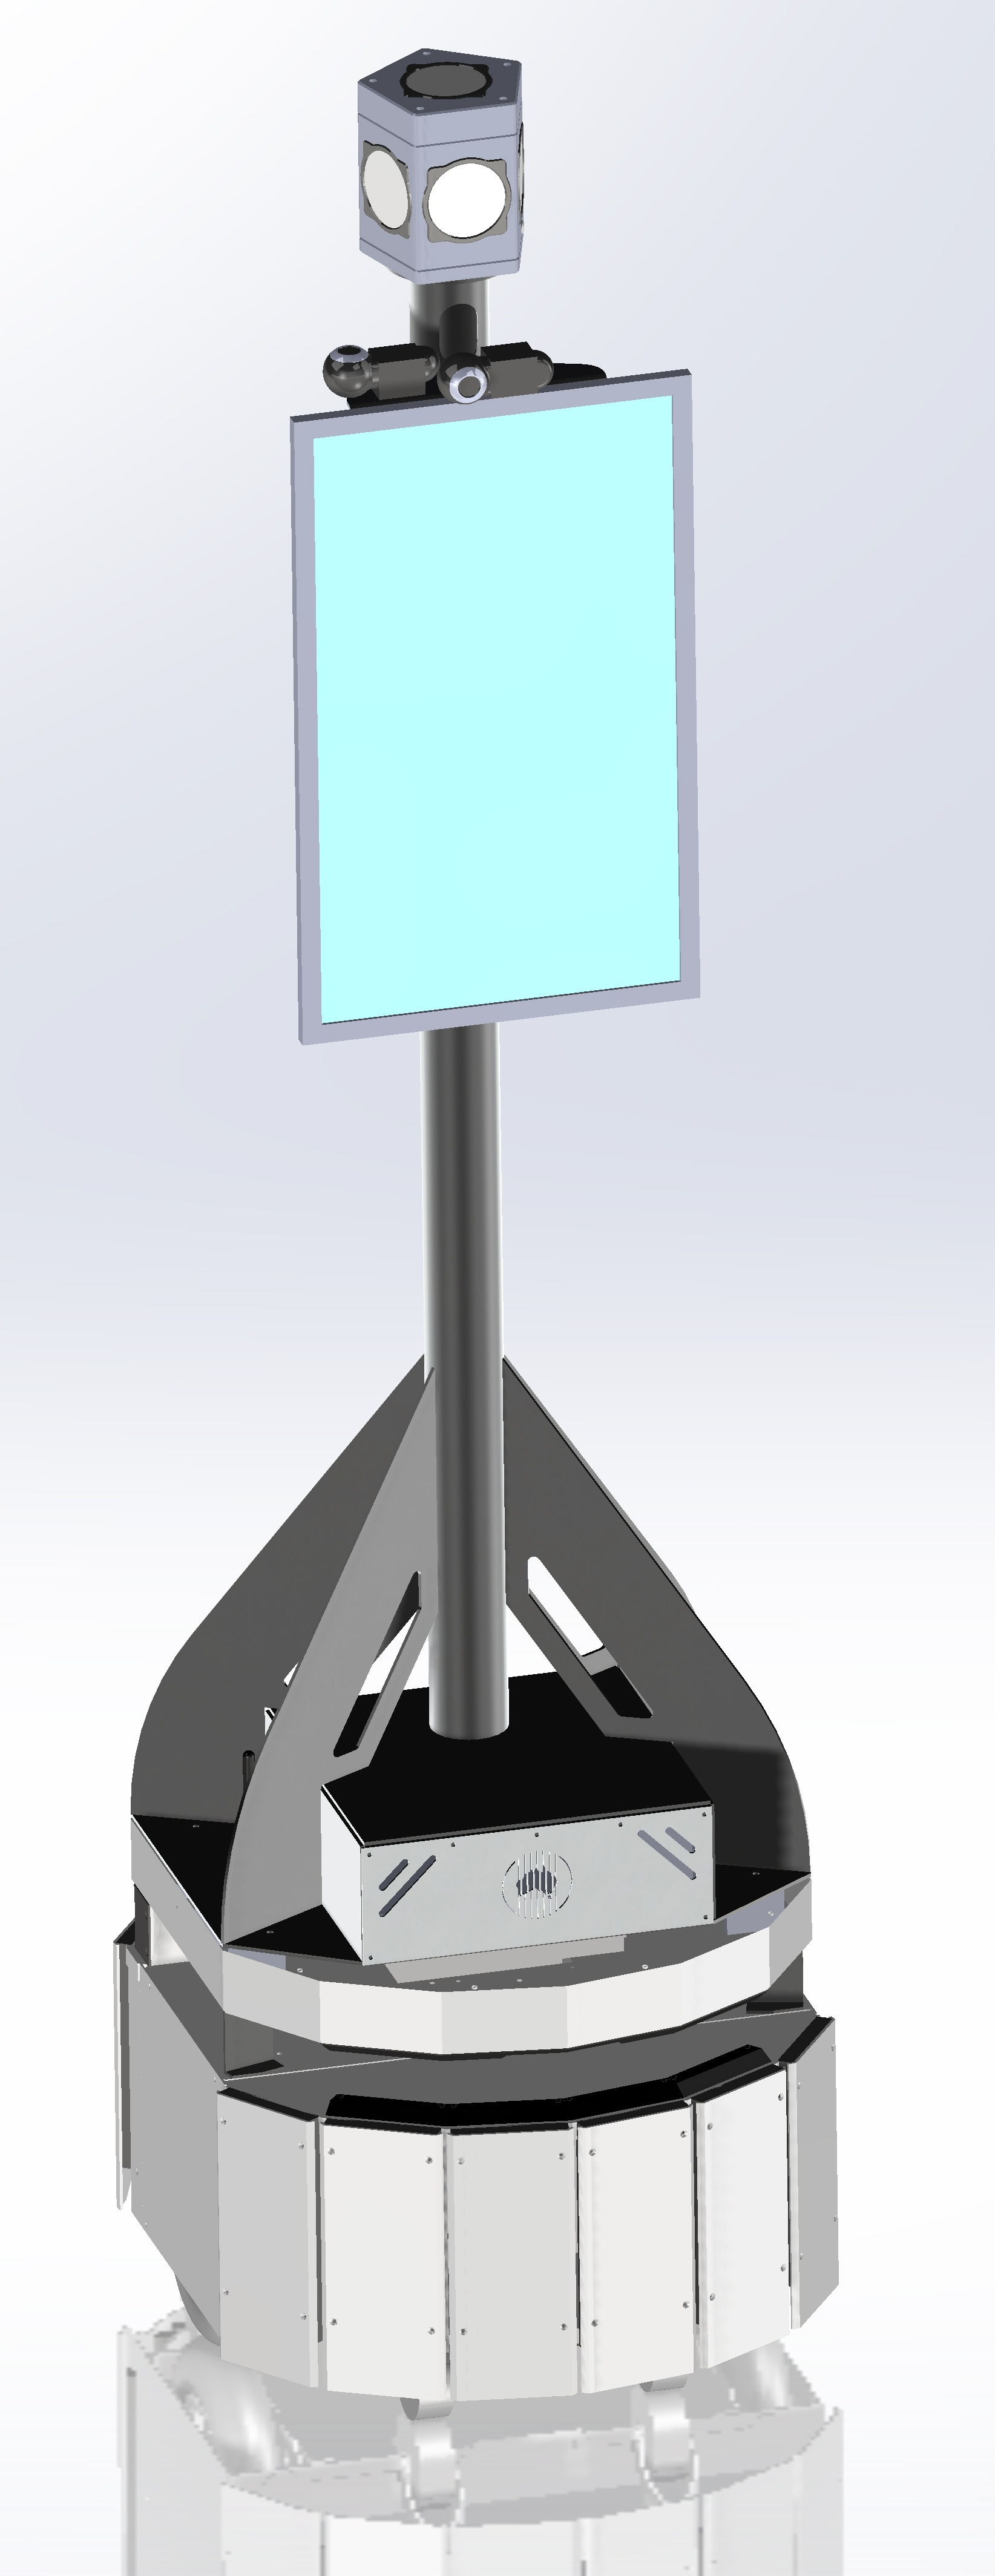
\includegraphics[width=0.25\textwidth, height=65mm]{figures/MuseumRobot.jpg}
 \end{center}
 %\fitbitmap{figures/ladybug.jpg}
 \caption{\textbf{Prototype of telepresence robot.} The figure displays the main components of the robot, a panoramic
 camera on its top, a screen in the middle and a mobile unit in the bottom.}
 \label{MuseumRobot}
\end{figure}

The robot moves at walking speed within any wheelchair accessible space. The robot is able to navigate
semi-autonomously to different locations in the museum under the supervision of the tour guide. Using light depiction
and ranging technology, the robot is able to detect walls, exhibits and people around and avoid them using a dynamic
obstacle avoidance system as part of its navigation system.  Hence, the robot can map its surroundings into a real-time
map of the gallery space that allows it to monitor its location in space.


\subsection{Museum Tour Guide}
The museum tour guide wears a wireless lapel microphone to ensure that he can be heard by the remote students while
carrying out a museum tour. The museum tour guide can see who is online and which students have questions via the
display on the front of the robot. With the proposed enhancement we are describing in this work, the museum guide is
also able to monitor the gaze of the remote visitors on the screen of the robot.


\subsection{360$^\circ$ Video and panoramic viewer}
A panorama is a single wide-angle image of the environment around the camera \cite{Gledhill2003435}. The most realistic
types surround the camera on the horizontal plane (360$^\circ$), and 180$^\circ$ in the vertical field of view. 
There are different ways to capture a panorama: single, rotated about its optical center, single omnidirectional camera
(using multiple cameras facing  in different directions) or using a stereo panoramic camera from which scene
information can be extracted.

The 360$^\circ$  panoramic camera (Figure \ref{ladybug}) used in our telepresence system was mounted on top of the robot
and captued a high-resolution omnidirectional image of the robot's environment. 

\begin{figure}[tp]
\begin{center}
 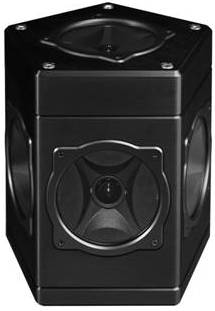
\includegraphics[width=0.25\textwidth, height=50mm]{figures/ladybug.jpg}
 \end{center}
 %\fitbitmap{figures/ladybug.jpg}
 \caption{The figure displays the ladybug 360$^\circ$ panoramic camera on top of the robot that uses several cameras
 facing different directions to create a panoramic image of the robots surroundings.}
 \label{ladybug}
\end{figure}


Several cameras capture multiple images of a scene from different viewpoints from which stereo information can be
calculated and then used to create a 3-D model of the scene in the form of a cubical or spherical panoramas, see Figures
\ref{panoramicImage} and \ref{omnidirectionalimage}.

\begin{figure}[tp]
 \begin{center}
 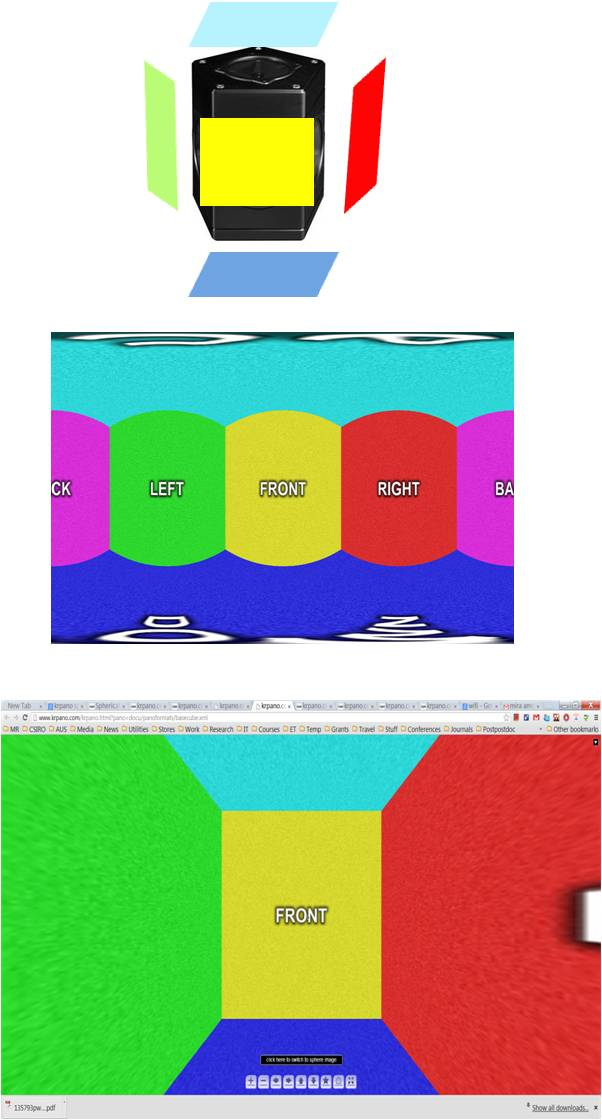
\includegraphics[width=0.45\textwidth, height=70mm]{figures/panoramicImage.jpg}
 \end{center}
 %\fitbitmap{figures/ladybug.jpg}
 \caption{\textbf{Creation of an Immersive Telepresence System.} The panoramic camera is used to capture several planes
 of the robot environment that are then stitched together in the panoramic viewer to create an immersive 3D-like
 experience for the remote users} 

 \label{panoramicImage}
\end{figure}

\begin{figure}[tp]
\begin{center}
 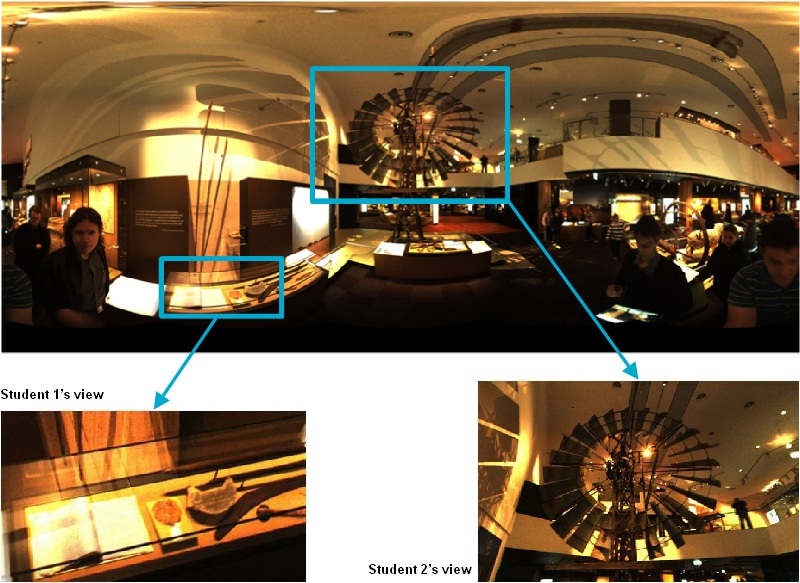
\includegraphics[width=0.45\textwidth, height=60mm]{figures/omnidirectionalimage.jpg}
 \end{center}
 %\fitbitmap{figures/ladybug.jpg}
 \caption{Images from the 360$^\circ$ camera on top of the robot are combined to form a high-resolution omnidirectional
 image that creates a 360$^\circ$ representation of the environment around the robot.}
 \label{omnidirectionalimage}
\end{figure}

The panoramic image viewer used in the remote computers was krpano\footnote{\url{http://krpano.com/}}. Krpano is a light
and very flexible high-performance viewer for all kind of panoramic images and interactive virtual tours. The viewer is
available as Flash and HTML5 application and is designed for the usage inside the Browser on Desktop and Mobiles
computer devices. Each remote students can then independently ``look around'' the gallery using the panoramic viewer
within their browser as shown in Figure \ref{museumtourview}.

\begin{figure}[tp]
 \fitbitmap{figures/museumtourview.jpg}
 \caption{Remote browser interface client through which student can look around the
museum with freedom to look at different areas within the 360 field of view environment}
 \label{museumtourview}
\end{figure}




\subsection{Remote Students' Client Computers}
Each student computer is equipped with a low cost eye tracker capturing gaze frames at 30Hz. The eye tracker provides
the X, Y coordinates of gaze on screen. Since the remote museum visitor can also control their horizontal and vertical
field of view within the panoramic camera, these parameters are also monitored by a javascript script running behind the
scenes in the browser. The horizontal and vertical view points refer to the views that determine the plane being
displayed on screen at any given time from the panoramic image. The combine parameters of horizontal, vertical field of
view and X, Y gaze coordinates are transformed in krpano into spherical coordinates to obtain the gaze point of regard
of the user in the spherical space. 


These four parameters define that define the point in 3D space the student is looking at are sent
back to the robot, see Figure \ref{aggregatedGazeBehavior}.

\begin{figure}[tp]
 \fitbitmap{figures/aggregatedGazeBehavior.jpg}
 \caption{Network of eye trackers on the remote students computer captures the gaze behavior of the students and
 combines the gaze data into a high-resolution omni-directional image}
 \label{aggregatedGazeBehavior}
\end{figure}

Images from the 360 degree camera on top of the robot are combined to form a condensed omni-directional image currently
being captured. The points of regard of several remote museum visitors are projected into this image to provide feedback
to the educator about where the students are paying attention to in the scene, see Figure \ref{aggregatedGazeBehavior}
and \ref{robotDisplay}.

\begin{figure}[tp]
 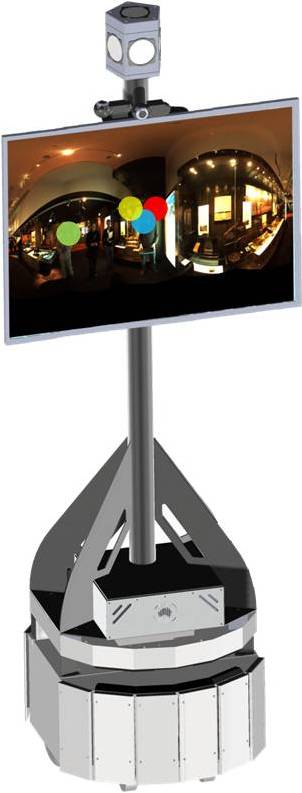
\includegraphics[width=0.4\textwidth, height=140mm]{figures/robotDisplay.jpg}
 \caption{Aggregated gaze behavior of remote
students superimposed into the omni-directional is shown in the robot display so the tour guide for instance can obtain
feedback about what areas in space the remote students are paying attention to}
 \label{robotDisplay}
\end{figure}


Each remote student computers uses a server-client arquitecture to gather the data being monitored. A javascript
client program embedded in the browser displayed paga monitors the panoramic viewer field of view and stream this
data through a websocket to a local server that also receives gaze coordinates from a gaze tracker
client. This server streams the horizonta and vertical field of view and the gaze coordinates to a further server located in the robot that
dispatches all the gaze data streams to a handler that displays this information on top of a condensed representation of
the omni-directional image currently being captured by the robot.

The TCP protocol is used to issue commands to the eye trackers such as start calibration, calculate results from
calibration, start tracking, stop tracking. Gaze estimation is sent through the UDP protocol, since the system can
afford to lose some packets since this would not impact the visualization of the gaze behavior of remote museum
visitors.


%---------------------------------------------------------------
\section{Application}
In order to gather sends about how their remote gaze monitoring system in the  robotic telepresence  scenario works,
the interested reader is encouraged to take a look at the manuscript's associated video at
\url{http://www.youtube.com/watch?v=gB89jT2_3oA}. The video provides a good visual overview of the system at work
and how it can be used to monitor the gaze behavior of remote museum visitors.


\section{Discussion}

National institutions such as museums have a responsibility to reach regional and remote school students who are often
unable to visit them physically due to factors such as cost and distance. A mobile telepresence system provides an
opportunity for regional and remote students to participate in visits to museums and other educationally relevant
institutions.


A key challenge for telepresence systems will how to leverage the new opportunities provided by telepresence
technology to engage students and stimulate learning.

The interactive nature of the systems permits interactive learning rather than passive and collaborative learning by
allowing students to interact with each other and with the tour guide.


System is immersive, ( remote students feel as if they are present in the gallery )
interactive ( remote students engage in discussions with the educator and other students on the tour )
Engaging ( students can explore digital content that is relevant to the current conversation)

Telepresence facilitates one region of the world exporting specialized skills to anywhere

Elimination of many chemical and physical health hazards

Reduction of transportation costs and of energy and commuting time

Importance of high quality sensory feedback

Time and cost benefits. The visual aspect greatly enhances communications, allowing for perceptions of facial
expressions and other body language.


At the present time, this is project is still a work in progressthat these currently testing  the  working  of  early
prototypes of the system but that has already  reached a proof of concept status. Future work can strive to carry out
 user studies to be carried involving students (ages 10-16) from several national high schools.
Their gaze could be monitored through a network of low cost Tobii Rex eye trackers. These eye trackers offer a
resolution of 30 samples per second and produce gaze estimation with an average accuracy of 0.5 degrees at 60
cm from the screen, enough for the no high resolution intensive application described here. 

Ones are but the form is in place highly sophisticated  studies about learning  can be envisioned. For instance, they
gaze behavior of a class of students could be monitor during the museum visit. After the visit, the students would be
required to answer a questionnaire  to measure the degree of understanding and acquired knowledge  that they acquired
through the visit. with these data in place, correlations between the gaze behavior  of  students performing poorly  on
the questionnaire and that of the students performing well could generate  interesting insights that could point out 
gaze dynamics specifics pointing towards student becoming disengaged with the task. once these knowledge would be in
place, it could be online to recapture the attention of students that the system detects that are starting to become
distracted.



\bibliography{library}
\end{document}

